\documentclass{article}
\usepackage[utf8]{inputenc}
\usepackage{geometry}
\usepackage{hyperref}
\usepackage{multicol}
\usepackage{graphicx}

 \geometry{
 a4paper,
 total={170mm,257mm},
 left=20mm,
 top=20mm,
 }
 \usepackage{graphicx}
 \usepackage{titling}

 \title{Group A3D: RDF Dataset}
\author{Group A3D}
\date{20th December 2024}

 \usepackage{fancyhdr}
\fancypagestyle{plain}{%  the preset of fancyhdr
    \fancyhf{} % clear all header and footer fields
    % \fancyfoot[R]{\includegraphics[width=2cm]{KULEUVEN_GENT_RGB_LOGO.png}}
    \fancyhead[]{\thedate}
    \fancyhead[L]{RDF Dataset}
    \fancyhead[R]{\theauthor}
}
\makeatletter
\def\@maketitle{%
  \newpage
  \null
  \vskip 1em%
  \begin{center}%
  \let \footnote \thanks
    {\LARGE \@title \par}%
    \vskip 1em%
    %{\large \@date}%
  \end{center}%
  \par
  \vskip 1em}
\makeatother

\usepackage{lipsum}
\usepackage{cmbright}

\begin{document}

\maketitle

\begin{tabular}{@{}ll}
	\textbf{Group members:}
	 & \href{mailto:andrea.bruttomesso.1@studenti.unipd.it}{Andrea Bruttomesso} 2120933 \\
	 & \href{mailto:alessandro.corro.1@studenti.unipd.it}{Alessandro Corr\`o} 2125034   \\
	 & \href{mailto:davide.seghetto@studenti.unipd.it}{Davide Seghetto} 2122548         \\
	 & \href{mailto:andrea.stocco.8@studenti.unipd.it}{Andrea Stocco} 2108885           \\
\end{tabular}
\\\\\\
\begin{tabular}{@{}ll}
	\textbf{Link to the GitHub repository:} \href{https://github.com/andreastocco01/a3d}{https://github.com/andreastocco01/a3d}
\end{tabular}

\section*{Ontology domain}
The domain of interest for our ontology focuses on scientific research. In particular, we aim to analyze potential correlations between Nobel Prize winners,
their publications, and the research funding allocated by nations. \\
Figure \ref{fig:nobelOntology} shows a schema of our ontology comprehensive of all the classes
and the properties modeled. For data integration we also imported well-known ontologies available on the web, such as \textit{SKOS}, \textit{FOAF} and \textit{EulerSharp countries}.

\begin{figure}[ht]
	\centering
	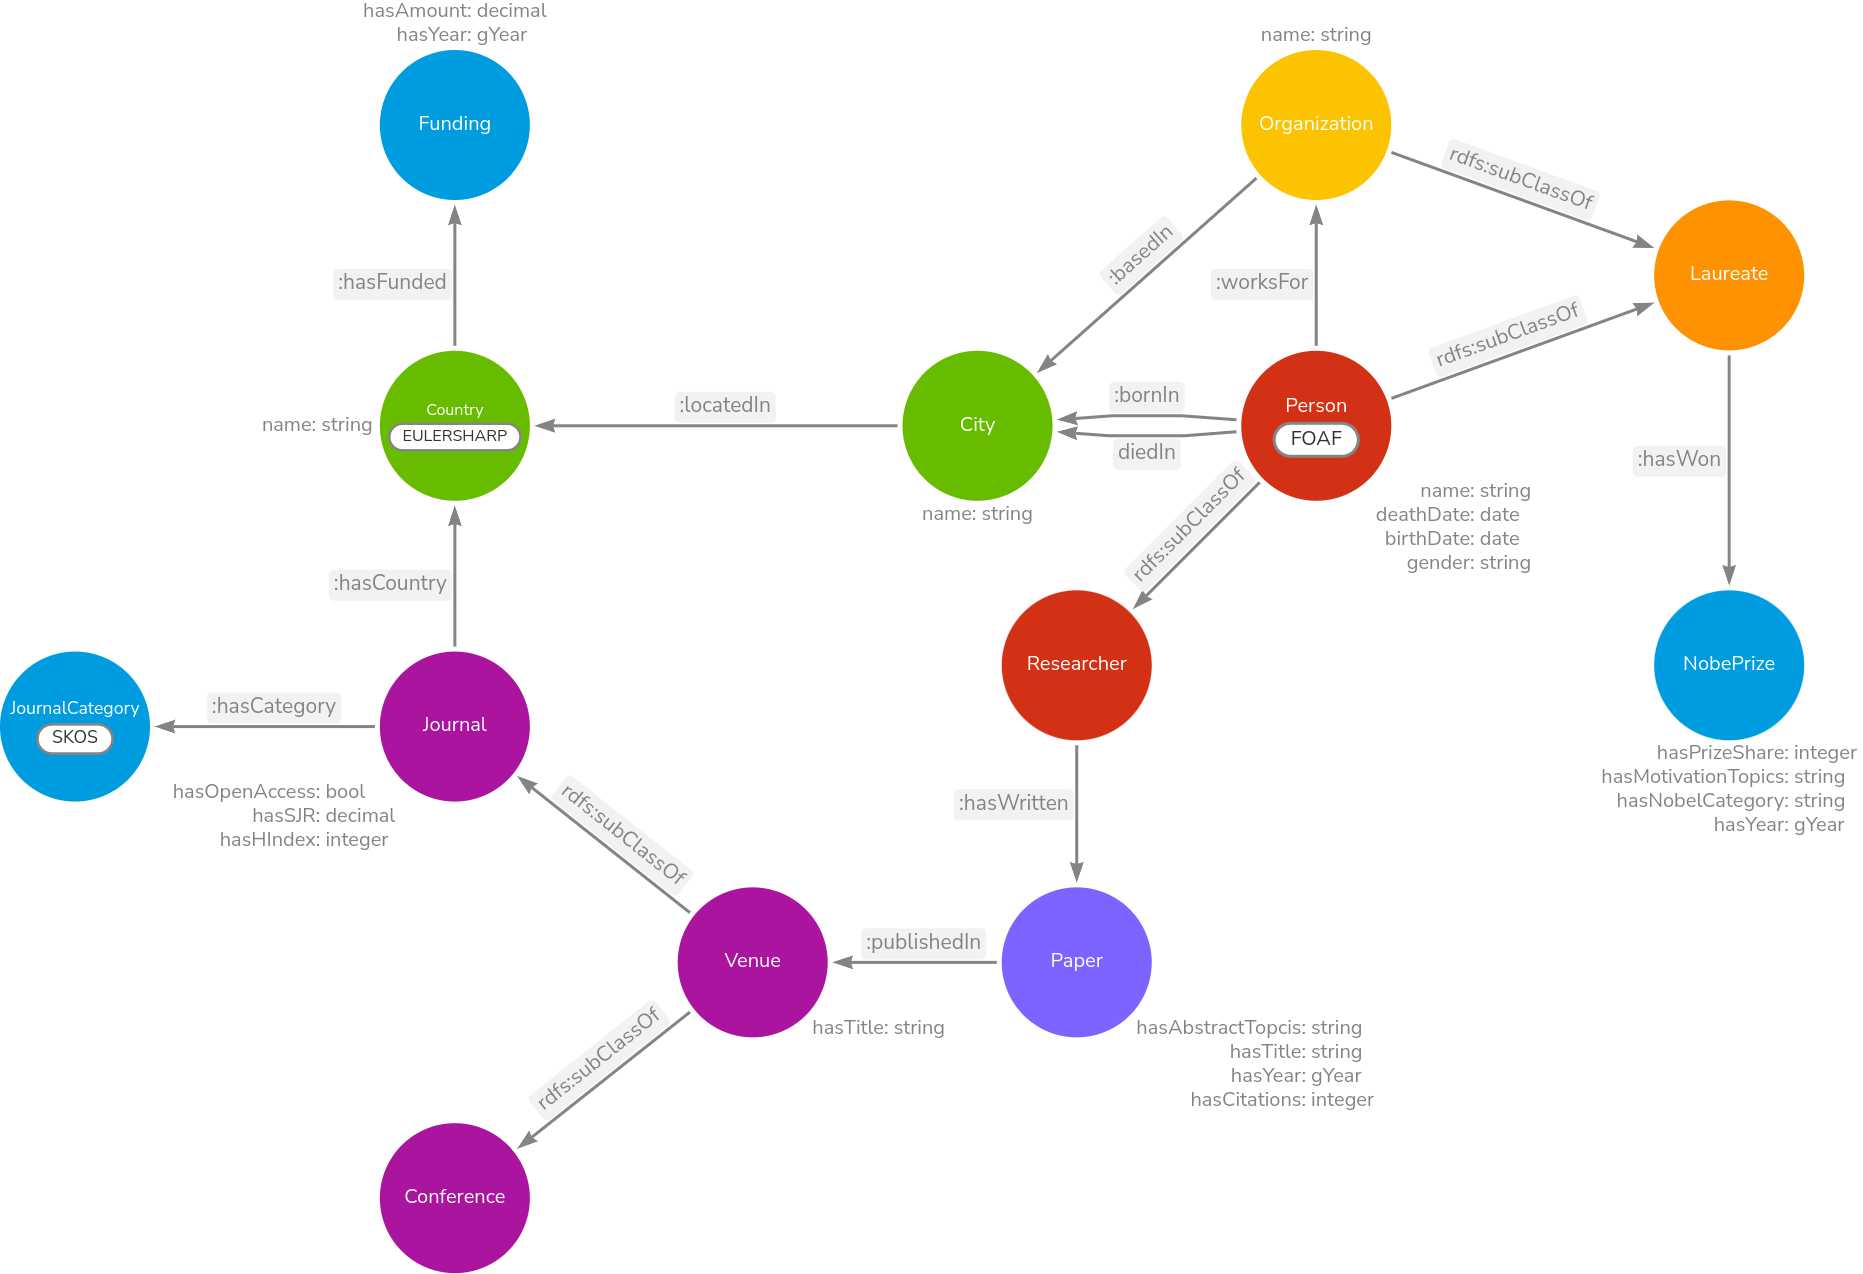
\includegraphics[width=\textwidth]{../nobelOntologyTransparent.png}
	\caption{Nobel Ontology}
	\label{fig:nobelOntology}
\end{figure}

\section*{Datasets and Population}
To populate our ontology, we used four distinct open datasets containing information about Nobel Prizes, scientific papers, publication venues and
national funding. The use of multiple datasets required us to address various inconsistencies. \\
Specifically, to resolve the discrepancies in names across the datasets,
we used the Python library \textit{rapidfuzz} for fuzzy matching the laureates' names with those of paper authors. We also ensured the absence of duplicates to
maintain data integrity. \\
Additionally, we encountered discrepancies with the EulerSharp ontology.
For instance, some country names in our datasets differed from those used in the EulerSharp ontology, such as "United
States" and "United States of America". These cases were manually addressed to ensure consistency. \\
Another critical aspect was filtering the information provided by various datasets. Initially, the Paper dataset contained 
over one million rows, making it necessary to reduce its size to avoid an excessively large and imbalanced 
database, particularly favoring the Researchers in terms of class population. To address this, we first selected 
only papers authored by Laureates or published in Journals also included in the dedicated dataset. 
Subsequently, we further narrowed it down to the first 50,000 rows of the already filtered dataset 
for the reasons outlined above.\\
Furthermore, we wrote a small script (\textit{topic\_extraction.py}) that uses \textit{gensim} to extract the most significant topics from lengthy textual properties.
For example, long descriptions such as "in recognition of the extraordinary services he has rendered by the
discovery of the laws of chemical dynamics and osmotic pressure in solutions" were reduced into more focused terms like "chemical dynamics osmotic
pressure solutions." This approach enhances the dataset's efficiency and significance while preserving its key concepts.

\section*{Main Statistics}

The following statistics summarize the key features of the RDF dataset.

\begin{itemize}
	\item	\textbf{Triples Count:}
				\begin{itemize}
				\item Total number of RDF triples: 3298916
				\end{itemize}
	\item	\textbf{Entities:}
				\begin{itemize}
		      	\item Number of unique entities:
		            \begin{itemize}
			            \item Person: 110981
			            \item Researchers: 110160
			            \item Laureates: 904 (23 Organizations, 881 Persons)
			            \item Organizations: 339
			            \item Papers: 53492
			            \item Journals: 18466
			            \item Conferences: 309
			            \item Cities: 874
			            \item Countries: 246
			            \item Nobel Prizes: 579
			            \item Funding: 1373
		            \end{itemize}
				\end{itemize}

	\item \textbf{Laureates and Nobel Prizes:}
	      \begin{itemize}
		      \item Researchers that won a Nobel Prize: 60
		      \item Total Nobel Prizes awarded: 969
		      \item Prize categories: 6 (Physics, Chemistry, Medicine, Literature, Peace, Economics)
	      \end{itemize}
	\item \textbf{Most Funding Countries: }
		\begin{enumerate}
			\item United States: \$4128 bn
			\item Japan: \$1189 bn
			\item Germany: \$1056 bn
		\end{enumerate}
	
\end{itemize}

\end{document}
